\documentclass[11pt,a4paper]{book}
\usepackage{float}
\usepackage{booktabs}
\usepackage{scrextend}
\usepackage[utf8]{inputenc}
\usepackage{amsmath,amsfonts,amssymb,bm,dsfont}	%Math fonts
\usepackage{amsthm}                         % Soporte matemático adicional
\usepackage{graphics}                       % Soporte gráfico
\usepackage{graphicx}                       % Soporte gráfico adicional
\usepackage{color,colortbl}                 % Creación de fondo y texto en color
\usepackage{geometry}                       % Soporte gr?fico
\usepackage{rotating}                       % Soporte gr?fico
\usepackage{enumerate}
\usepackage{textcomp}
\usepackage{cite}
\usepackage{subcaption}
\usepackage{titlesec}
\usepackage{fancyhdr}
\usepackage[T1]{fontenc}
\usepackage{epsfig}
\usepackage[percent]{overpic}
\usepackage{listings}
\usepackage[normalem]{ulem}
\usepackage[bottom]{footmisc}
\usepackage{pifont}
\usepackage[pdfstartview=FitB,pdfstartpage=1,backref=true]{hyperref}
\hypersetup{
	colorlinks=true,
	pdfborder={0 0 0},	    
	linkcolor={red},
	citecolor={blue!85!black},
	urlcolor={blue!80!black}
}
\usepackage{makeidx}
\usepackage[nottoc,notlot,notlof]{tocbibind} %Para incluir la bibliografía y el índice
\usepackage{times}  
\usepackage{float}
\usepackage{epsfig}
\usepackage[percent]{overpic}
\usepackage{listings}
\usepackage[normalem]{ulem}
\usepackage[bottom]{footmisc}
\usepackage{pifont}

\documentclass{report}

\usepackage{titlesec}
\titleformat{\chapter} % Not to print Chapter headings
  {\Large\bfseries} 
  {}                
  {0pt}             
  {\huge}

\begin{document}
	\thispagestyle{empty}

\begin{figure}[H]
    \centering
    
\includegraphics[scale=0.9]{MPNG_logo.eps}
\end{figure}

\vspace{0.5cm}

\begin{center}
	\LARGE \textbf{User's Manual}
\end{center}

\vspace{0.5cm}

\begin{center}
	\Large Version 0.99a
\end{center}

\vspace{1cm}


\begin{table}[H]
	\centering
	\begin{tabular}{lcr}
		Sergio García-Marín & Wilson González-Vanegas & Carlos E. Murillo-Sánchez
	\end{tabular}
\end{table}

\vspace{0.5cm}
\begin{center}
	\today
\end{center}
		
\vspace{9cm}

\begin{center}
	{\footnotesize \textcopyright $\;$ Definir con el profe qué va aquí.}
\end{center}

\newpage
	\addtocontents{toc}{\vspace{-4ex}}
	\tableofcontents                            
	\listoffigures
	\listoftables
	
	\normalsize
\pagenumbering{arabic}
\setcounter{page}{1}

\chapter{Introduction}
\label{chap:intro}

\section{Background}
\label{sec:background}

\mpng{} is a \matpower{}-based~\cite{zimmerman2011,matpower} package for solving optimal power and natural gas flow problems. \mpng{} uses the general user nonlinear constraints capability of \matpower{} to model the gas network taking into account gas-fired power generators, storage units, wells, power-and-gas-driven compressors, and nodes with stratified demand (different market segments get different priorities). The \mpng{} source code can be found at:

\bigskip
~~~~~~~~~~~~~~~~~~~~~~\url{\mpngurl}
\bigskip

\noindent \mpng{} was developed by Sergio~García-Marín~\footnote[1]{ Universidad Nacional de Colombia - sede Manizales.\label{foot:UNAL}} and Wilson~González-Vanegas~\footnote[2]{ Universidad Tecnológica de Pereira.\label{foot:UTP}} under the direction of Professor Carlos~E.~Murillo-S\'anchez~\footref{foot:UNAL}. The initial need for a \matpower{}-based power and natural gas optimal flow package was born out of a project aimed at analyzing the integrated operation of the Colombian power and natural gas systems.\footnote[3]{ Project number 1110-745-58696 funded by Colciencias, Colombia.}

\section{License and Terms of Use}
\label{sec:license}

As a \matpower{}-based package, \mpng{} is distributed under the 3-clause BSD license~\cite{bsd}. The full text of the license can be found in the \code{LICENSE} file at the top level of the distribution or at \url{https://github.com/MATPOWER/mpng/blob/master/LICENSE} and reads as follows. 

\begin{Notice}
Copyright (c) 2019, individual contributors (see AUTHORS file for 
details). All rights reserved.

Redistribution and use in source and binary forms, with or without
modification, are permitted provided that the following conditions
are met:

1. Redistributions of source code must retain the above copyright
notice, this list of conditions and the following disclaimer.

2. Redistributions in binary form must reproduce the above copyright
notice, this list of conditions and the following disclaimer in the
documentation and/or other materials provided with the distribution.

3. Neither the name of the copyright holder nor the names of its
contributors may be used to endorse or promote products derived from
this software without specific prior written permission.

THIS SOFTWARE IS PROVIDED BY THE COPYRIGHT HOLDERS AND CONTRIBUTORS
"AS IS" AND ANY EXPRESS OR IMPLIED WARRANTIES, INCLUDING, BUT NOT
LIMITED TO, THE IMPLIED WARRANTIES OF MERCHANTABILITY AND FITNESS
FOR A PARTICULAR PURPOSE ARE DISCLAIMED. IN NO EVENT SHALL THE
COPYRIGHT HOLDER OR CONTRIBUTORS BE LIABLE FOR ANY DIRECT, INDIRECT,
INCIDENTAL, SPECIAL, EXEMPLARY, OR CONSEQUENTIAL DAMAGES (INCLUDING,
BUT NOT LIMITED TO, PROCUREMENT OF SUBSTITUTE GOODS OR SERVICES;
LOSS OF USE, DATA, OR PROFITS; OR BUSINESS INTERRUPTION) HOWEVER
CAUSED AND ON ANY THEORY OF LIABILITY, WHETHER IN CONTRACT, STRICT
LIABILITY, OR TORT (INCLUDING NEGLIGENCE OR OTHERWISE) ARISING IN
ANY WAY OUT OF THE USE OF THIS SOFTWARE, EVEN IF ADVISED OF THE
POSSIBILITY OF SUCH DAMAGE.
\end{Notice}

\section{Citing MPNG}
\label{sec:citing_MPNG}

While not required by the terms of the license, we do request that publications derived from the use of \mpng{} explicitly acknowledge that fact by citing this manual~\cite{mpng2019}. In the near future, a journal publication to appear should be cited instead.

\begin{quote}
	\small
	S.~García-Marín, W.~González-Vanegas, and C.~E. Murillo-Sánchez, ``MPNG: \matpower{}-Natural Gas,'' 2019.
	[Online]. Available: \url{\mpngurl}
\end{quote}
	\chapter{Getting started}
\label{chap:get_started}

\section{System Requirements}
\label{sec:requirements}

To use \mpng{} you will need the following system requirements:

\begin{itemize}
	\item[\checkmark] \matlab{}\textsuperscript{\tiny \textregistered} version 7.3 (R2016b) or later.\footnote{\matlab{} is available from The MathWorks, Inc. (\url{https://www.mathworks.com/}). An R2016b or later \matlab{} version is required as the \mpng{} code uses \matlab{}-files with multiple function declarations.}
	
	\item[\checkmark] \matpower{} version 7.0 or later.\footnote{\matpower{} is available thanks to the Power Systems Engineering Research Center (\pserc) (\url{https://matpower.org})}
\end{itemize}

\section{Getting \mpng{}}
\label{sec:get_mpng}

You can obtain the \emph{current development version} from the \matpower{} Github repository: \url{https://github.com/MATPOWER/mpng.git}.


\section{Running a Simulation}
\label{sec:simulate}

The primary functionality of \mpng{} is to solve optimal power and natural gas flow problems. Running a simulation using \mpng{} requires (1) preparing the natural gas input data, (2) specifying the interconnection input data to couple the gas network to the power system, (3) invoking the function to run the integrated simulation and (4) accessing and viewing the results.\\

The classical \matpower{} input data is a ``\matpower{}-case'' struct denoted by the variable \code{mpc}\cite{matpower_manual}. To integrate the power and natural gas systems we use the extended Optimal Power Flow (OPF) capability of \matpower{}. Namely, we model the natural gas system and its connection to the power system via general user nonlinear constrains. Then, \mpng{} uses an extended ``\matpower{}-gas case'' struct denoted by the variable \code{mpgc}. In particular, \code{mpgc} is a traditional \matpower{}-case struct with two additional fields, \code{mpgc.mgc} and \code{mpgc.connect} standing for the natural gas case and interconnection case, respectively.

\subsection{Preparing the Natural Gas Case}
\label{subsec:gas_case}

The input data of the natural gas system are specified in a set of matrices arranged in a \matlab{} struct that we refere to as the ``gas case'' (\code{mpgc.mgc}). The structure of such a gas case is formatted in a similar way to the \matpower{}-case but holding the natural gas information that comprise gas bases, nodes, wells, pipelines, compressors, and storage units. See Appendix~\ref{app:gas_format} for more details about the gas case structure.

\subsection{Connecting the Gas Case to the \matpower{} Case}
\label{subsec:connect_case}

The input data regarding the connection between the power and natural gas systems are declared in a set of matrices packaged as a \matlab{} struct which we call ``interconnection case'' (\code{mpgc.connect}). The structure of this case contains specific information about coupling elements as gas-fired power generators and power-and-gas-driven compressors, according to the optimization model described in section~\ref{chap:formulation}. See appendix~\ref{app:connect_format} for more details about the interconnection case structure.

\subsection{Solving the Optimal Power-Gas Flow}
\label{subsec:solve_OPGF}

Once the \matpower{}-gas case is properly formatted, one can invoke the solver using the (mandatory) \code{mpgc} struct and the traditional (optional) \matpower{} options struct \code{mpopt}. The calling syntax at the \matlab{} prompt is as follows:  

\begin{Code}	
>> results = mpng(mpgc,mpopt);
\end{Code}

For more details, type:

\begin{Code}
>> help mpng
\end{Code}






	\chapter{Formulation}
\label{chap:formulation}

\section*{Nomenclature}
\subsection*{Indexes}
\begin{labeling}{alligator}
\item [$i$, $j$] Gas nodes.
\item [$m$, $n$] Electric nodes (buses). 
\item [$o$] Gas pipeline.
\item [$c$] Compressor.
\item [$l$] Transmission line.
\item [$w$] Gas well.
\item [$e$] Power generator.
\item [$ref$] Reference bus.
\item [$r$] Spinning reserve.
\item [$\sigma$] Type of gas load.
\end{labeling}

\subsection*{Parameters}

\begin{labeling}{alligator}

\item [$\alpha^{i}_{\pi_+}, \alpha^{i}_{\pi _-}$] Penalties for over-pressure and under-pressure at node $i$.
\item [$\alpha_{\gamma}$] Penalties for non-supplied gas.
\item [$\alpha_{\epsilon}$] Penalties for non-supplied electricity.
\item [$C^{w}_{G}$] Gas cost at the well $w$.
\item [$C^{oij}_{O}$] Transport cost of pipeline $o$, from node $i$ to node $j$.
\item [$C^{cij}_{C}$] Compression cost of compressor $c$, from node $i$ to node $j$.
\item [$C^{i}_{S}$] Storage cost at node $i$.
\item [$C^{i}_{S_+}$] Storage outflow price at node $i$.
\item [$C^{i}_{S_-}$] Storage inflow price at node $i$.
\item [$C^{e}_{E}$] Power cost generation (excluding gas cost).
\item [$\eta^{q}_{e}$] Thermal efficiency at generator $q$ \textit{[MMSCF/MW]}.
\item [$D_{g}^{i \sigma}$] Gas demand of type $\sigma$ at node $i$.
\item [$D_{e}^{tm}$] Electricity demand in the bus $m$ at time $t$.
\item [$\bar{g}^{w}$, $\underline{g}^{w}$] Gas production limits.
\item [$\overline{\pi}^{i}$, $\underline{\pi}^{i}$] Quadratic pressure limits at node $i$.
\item [$S^{i}_{0}$] Initial stored gas at node $i$.
\item [$\overline{S}^{i}$, $\underline{S}^{i}$] Storage limits at node $i$.
\item [$\kappa^{oij}$] Weymouth constant of pipeline $o$.
\item [$\delta^{oij}$] Width for gas flow capacities.
\item [$\beta^{cij}$] Compression ratio of compressor $c$.
\item [$Z^{c}$] Ratio parameter of compressor $c$.
\item [$B^{c}$] Compressor design parameter of compressor $c$.
\item [$x$, $y$, $z$] Gas consumption parameters of gas-fired compressors.
\item [$\overline{f}^{oij}_{g}$] Gas transport capacity of pipeline $o$, from node $i$ to node $j$.
\item [$\overline{f}^{cij}_{g}$] Gas flow capacity of compressor $c$, from node $i$ to node $j$.
\item [$\overline{f}^{i}_{s}$,$\underline{f}^{i}_{s}$] Storage outflow capacities at node $i$.
\item [$\overline{p}_{g}^{e}$, $\underline{p}_{g}^{e}$] Active power generation limits of generator $e$.
\item [$\overline{q}_{g}^{e}$, $\underline{q}_{g}^{e}$] Reactive power generation limits of generator $e$.
\item [$\overline{V}^{tm} \underline{V}^{tm}$] Voltage limits for every bus $m$ at time $t$.
\item [$\mathbb{S}^{l}$] Transmission capacity of power line $l$.
%\item [$x^{mn}_{l}$] Reactance of line $l$, from bus $m$ to bus $n$.
\item [$R^{tr}$]  Spinning reserve in the $r$-th spinning reserve zone at time $t$.
\item [$M$] Generators assignment matrix.
\item [$L$] Compressors assignment matrix.
\item [$u^{te}$] Unit commitment state for generator $q$ at time $t$.
\item [$\tau^{t}$] Energy weight related to period of time $t$.
\item [$E^{e}$] Available energy for hydroelectric generator $e$, \break during the total analysis window.

\end{labeling}

\subsection*{Sets}

\begin{labeling}{alligator}
\item [$\cal{N}$] Gas nodes, $\left| \cal{N} \right|= n_{\cal{N}}$.
\item [$\cal{N}_{S}$] Gas nodes with storage, $\cal{N}_{S} \subset \cal{N} $, $\left| \cal{N}_{S} \right|= n_{\cal{S}}$.
\item [${\cal{O}}$] Gas pipelines, $\left| \cal{O}  \right| = n_{\cal{O}}$
\item [${\cal{C}}$] Compressors, $\left| \cal{C}  \right| = n_{\cal{C}}$ 
\item [${\cal{C}}_{G}$] Compressors based on natural gas, ${\cal{C}}_{G} \subseteq {\cal{C}}$,   \hspace{5mm}   $\left| {\cal{C}}_{G}  \right| = n_{{\cal{C}}_{G}}$ 
\item [${\cal{C}}_{E}$] Compressors based on electric power, ${\cal{C}}_{E} \subseteq {\cal{C}}$,   \hspace{5mm}  $\left| {\cal{C}}_{E}  \right| = n_{{\cal{C}}_{P}}$ 
\item [${\cal{W}}$] Gas wells, $\left| \cal{W} \right|= n_{\cal{W}}$.
\item [${\cal{W}}^{i}$] Gas wells at node $i$, ${\cal{W}}^{i} \subset \cal{W} $, $\left| {\cal{W}}^{i} \right|= n_{{\cal{W}}^{i}}$.
\item [$\cal{B}$] Power buses, $\left| \cal{B} \right|= n_{\cal{B}}$.
\item [$\cal{L}$] Power lines, $\left| \cal{L} \right|= n_{\cal{L}}$.
\item [$\cal{E}$] Power unit generators, $\left| \cal{E} \right|= n_{\cal{E}}$.
\item [${\cal{E}}_{H}$] Hydroelectric power units, ${\cal{E}}_{H} \subseteq \cal{E} $, $\left| {\cal{E}}_{H} \right|= n_{{\cal{E}}_{H}}$.
\item [${\cal{E}}^{i}_{G}$] Gas-fired power units connected to gas node $i$, \break ${\cal{E}}^{i}_{G} \subseteq \cal{E}$, $\left| {\cal{E}}^{i}_{G} \right|= n_{{\cal{E}}_{G}}$.
\item [${\cal{Z}}_{r}$] Spinning reserve zones. 
\item [${\cal{F}}^{i}_{G}$, ${\cal{T}}^{i}_{G}$] Connected pipelines to node $i$ at side \textit{From} or \textit{To}.
\item [${\cal{F}}^{i}_{C}$, ${\cal{T}}^{i}_{C}$] Connected compressors to node $i$ at side \textit{From} or \textit{To}.
\item [${\cal{F}}^{m}_{E}$, ${\cal{T}}^{m}_{E}$] Connected power lines to bus $m$ at side \textit{From} or \textit{To}. 
\item [$\cal{T}$] Total periods of analysis.
\item [$\Sigma$] Different types of gas loads.
\end{labeling}


\subsection*{Variables}

\begin{labeling}{alligator}
\item [${f}_{g}^{oij}$] Gas flow in pipeline $o$, from node $i$ to node $j$.
\item [${f}_{g_+}^{oij}$ ${f}_{g_-}^{oij}$] Positive and negative gas flow in pipeline $o$.
\item [${f}_{g}^{cij}$] Gas flow in compressor $c$, from node $i$ to node $j$.
\item [$\psi^{c}$] Power consumed by compressor $c$.
\item [$\phi^{c}$] Gas consumed by compressor $c$, connected to node $i$ at side \textit{From}.
\item [$\gamma^{i \sigma}$] Non-served gas of type $\sigma$ at node $i$.
\item [$\pi^{i}$] Quadratic pressure.
\item [${\pi}^{i}_{+}$, ${\pi}^{i}_{-}$] Over/Under quadratic pressures at node $i$.
\item [$g^{w}$] Gas production at well $w$.
\item [$f_{s}^{i}$] Storage outflow difference.
\item [$f_{s_+}^{i}$, $f_{s_-}^{i}$] Storage outflow and inflow.
\item [$p_{g}^{te}$] Active power production at generator $q$ at time $t$.
\item [$q_{g}^{te}$] Reactive power production at generator $q$ at time $t$.
\item [$V^{tm}$] Voltage magnitude at bus $m$ at time $t$.
\item [$\theta^{tm}$] Voltage angle at bus $m$ at time $t$.
\item [$\epsilon^{tm}$] Non-served active power at bus $m$ at time $t$.
\end{labeling}






We made a toolbox and we want to explain how it works.

\section{Objective function}

%The cost function is represented by the equation \ref{obj_func} and is composed by several linear components. The first component is the gas production cost at each of the wells. As well as the first component, the second one is the power generation cost for every power plant, for the complete period. \color{red}The third component is the cost of the storage flow at every node with storage availability. \color{black}The fourth  expression is the storage cost, having into account the previous storage level and the outing flow. The fifth component is the gas transport cost for each pipeline. Finally, the last three component are the penalties cost for over/under pressure, non-supply gas and non-supply power, respectively. Related to the non-gas supply, is important to clarify that the non-supply cost depends on the type of user. 

\begin{equation}
\begin{aligned}
C \left( x \right) = & \sum_{w \in \cal{W}}{C^{w}_{G} g^{w}} + \sum_{t \in \cal{T}} {\tau}^{t}  \sum_{e \in \cal{E}} {C^{e}_{E} p_{g}^{te}}\\ 
				& + \sum_{i \in {\cal{N}}_{S}}{\left({C^{i}_{S_+} f^{i}_{s_+}} - {C^{i}_{S_-} f^{i}_{s_-}}  \right)}\\
				& + \sum_{i \in {\cal{N}}_{S}}{C^{i}_{S} \left( S^{i}_{0} - f^{i}_{s} \right)} \\
				& + \sum_{o \in \cal{O}}{C^{oij}_{O} f^{oij}_{g_+}} - \sum_{o \in \cal{O}}{C^{oij}_{O} f^{oij}_{g_-}} \\
				& + \sum_{c \in \cal{C}}{C^{cij}_{C} f^{cij}_{g}} \\ 
				& + \sum_{i \in \cal{N}}{\alpha^{i}_{\pi_+} \pi^{i}_{+}} + \sum_{i \in \cal{N}}{ \alpha^{i}_{\pi_-} \pi^{i}_{-}} \\
				& + \sum_{i \in \cal{N}}\sum_{\sigma \in \Sigma} {\alpha_{\gamma}^{i \sigma}\gamma^{i \sigma}} + \alpha_{\epsilon} \sum_{t \in \cal{T}} {\tau}^{t} \sum_{m \in \cal{B}} {\epsilon^{tm}}  
\end{aligned}
\label{obj_func}
\end{equation}

\section{Constraints}

\subsection{Gas network}

%The equation \ref{node_gas_balance} shows the gas balance for a specific node $k$ during a day. This gas balance is composed by the ingoing and outgoing flows at the node $k$, the related generation to that node, the outgoing stored flow in the available storage, and the total gas demand. The gas demand is composed by the demand required in the gas-fired power plants, and the total gas demand of the rest of the consumers, but excluding the non-supply gas. 

\begin{equation}
\begin{aligned}
& \sum_{o \in {\cal{T}}^{k}_{G}}{{f}_{g}^{oij}} - \sum_{o \in {\cal{F}}^{k}_{G}}{{f}_{g}^{oij}} + \sum_{c \in {\cal{T}}^{k}_{C}}{{f}_{g}^{cij}} - \sum_{c \in {\cal{F}}^{k}_{C}}{ \left({f}_{g}^{cij} + \phi^{c}\right)} \\
& + \sum_{w \in {\cal{W}}^{k}}{g^{w}}  + {f}^{k}_{s} - \sum_{t \in \cal{T}} {\tau}^{t} \sum_{e \in {\cal{E}}^{k}_{G}}\left({\eta^{q}_{e}}\cdot {p_{g}^{te}}\right) = {\sum_{\sigma \in \Sigma}\left( D^{\sigma k}_{g} - \gamma^{\sigma k}\right)} \\
& \forall k \in \cal{N}
\end{aligned}
\label{node_gas_balance}
\end{equation}

The non-supply gas demand in every node of the system can only be as most as the total demand at the same node. This constraint is represented as follows:

\begin{equation}
{0 \le \gamma^{\sigma k} \le D^{\sigma k}_{g} \quad \forall \sigma \in \Sigma \quad \forall k \in \cal{N}}
\label{nsg_limits}
\end{equation}

%The storage outflow difference is the subtraction between the storage outflow and the storage inflow at the storage nodes, this relationship is represented by equation \ref{fs}. Additionally, the outflow storage difference is restricted by the maximum and minimum amount of gas that is allowed to be injected into the network in every storage node, which is formulated in equation \ref{fs_limits}. As the storage can be either an injection or a demand for the network, equations \ref{fs+} and \ref{fs-} represent the behavior of the fluxes as follows, the maximum amount of natural gas that can be injected into the network by the storage, is the difference between the available natural gas and the minimum possible amount of gas that can remain. In the same sense, the maximum amount of natural gas that can be delivered by the network to the storage deposit, is the difference between the maximum natural gas that can be stored and the available natural gas.

\textbf{Storage}

\begin{equation}
f_{s}^{k} = f_{s_+}^{k}  - f_{s_-}^{k}\quad \forall k \in \cal{N}
\label{fs}
\end{equation}
\begin{equation}
\underline{f}^{k}_{s} \le f^{k}_{s} \le \overline{f}^{k}_{s} \quad \forall k \in \cal{N}
\label{fs_limits}
\end{equation}
\begin{equation}
0 \le f_{s_+}^{i} \le S^{k}_{0}  - \underline{S}^{k} \quad \forall k \in \cal{N}
\label{fs+}
\end{equation}
\begin{equation}
0 \le f_{s_-}^{i} \le \overline{S}^{k} - S^{k}_{0} \quad \forall k \in \cal{N}
\label{fs-}
\end{equation}

\textbf{Wells}\\

The constraints related to the gas wells production depends on each well specific characteristics, these constraints are represented by:

\begin{equation}
\underline{g}^{w} \le g^{w} \le \overline{g}^{w} \quad \forall w \in \cal{W}
\label{g_limits}
\end{equation}
%\vspace{5cm}

\textbf{Pipelines:} \\
%Equations \ref{gf_limits} to \ref{presa_rel} correspond to the constraints in passive and  pipelines. Weymouth equation is represented by \ref{wey_eq} and it determines the flow between two nodes, $i$ and $j$, in function of its pressure differences. The gas flow limits for passive pipelines are represented by \ref{gf_limits}. Otherwise, for active pipelines in which their flows is restricted to go only in one direction, the constraints are represented by \ref{gfa_limits}. Equation \ref{presa_rel} shows the linear relation between the pressure in two nodes connected by an active pipeline, this relation is modeled by a linear factor which depends on the characteristics of the compressor pipeline. 

\begin{equation}
{f}^{oij}_{g} = {{\kappa}^{oij}} sgn \left(\pi^{i}-\pi^{j}\right) {\sqrt{\left|\pi^{i}-\pi^{j}\right|}} \quad \forall o \in {\cal{O}}
\label{wey_eq}
\end{equation}

And the gas flow limits for every pipeline:

\begin{equation}
{f}^{oij}_{g} =  f^{oij}_{g_+} + {f}^{oij}_{g_-} \quad \forall o \in {\cal{O}}
\label{fgo}
\end{equation}
\begin{equation}
 - \overline{f}^{oij}_{g}  \le f^{oij}_{g} \le  \overline{f}^{oij}_{g}  \quad \forall o \in {\cal{O}}
\label{fgo_limits}
\end{equation}
\begin{equation}
0 \le f^{oij}_{g_+} \le \delta^{oij} \cdot \overline{f}^{oij}_{g} \quad \forall o \in {\cal{O}}
\label{fgopos_limits}
\end{equation}
\begin{equation}
- \delta^{oij} \cdot \overline{f}^{oij}_{g} \le f^{oij}_{g_-} \le 0 \quad \forall o \in {\cal{O}}
\label{fgoneg_limits}
\end{equation}



\textbf{Compressors:}\\

The power consumed by the compressors depend on its gas flow:\\

\begin{equation}
\psi^{c} = {B^{c}}{f}^{cij}_{g} \cdot \left( {\left( \frac{\pi^{j}}{\pi^{i}} \right)}^{Z^{c} / 2} - 1 \right)   \quad \forall c \in {\cal{C}}
\label{hp_fc}
\end{equation}
\begin{equation} 
{\phi}^{c} = x + y \psi^{c} +  z {\psi^{c}}^{2}  \quad \forall c \in {\cal{C}}_{G}
\label{g_fc}
\end{equation}
\begin{equation}
0 \le {f}^{cij}_{g} \le \overline{f}^{cij}_{g}  \quad \forall c \in {\cal{C}}
\label{gfa_limits}
\end{equation}
\begin{equation}
\begin{aligned}
&\pi^{i} \le \pi^{j} \le \beta^{cij} \pi^{i}\\
&\beta^{cij} \ge 1 \\
\end{aligned}
\quad \forall i,j \in {\cal{N}} \quad \forall c \in {\cal{C}}
\label{presa_rel}
\end{equation}
\\

The equations \ref{overp} and \ref{underp} are the constraints that characterize the quadratic overpressure and underpressure at every node of the system, respectively. 

\begin{equation}
\begin{array}{l}
 \pi^{k} \le \overline{\pi}^{k} + \pi^{k}_{+}\\
 0 \le \pi^{k}_{+}\\
\end{array} 
\quad \forall k  \in {\cal{N}}\\ 
\label{overp}
\end{equation}

\begin{equation}
\begin{array}{l}
\underline{\pi}^{k} - \pi^{k}_{-} \le \pi^{k}\\
0 \le \pi^{k}_{-}\\
\end{array} 
\quad \forall k  \in {\cal{N}}\\ 
\label{underp}
\end{equation}
\\

\subsection{Power network}

Equation \ref{power_balance} could be explained in an appendix section.
 
\begin{equation}
\begin{array}{l}
g_{p_m}\left(\theta^{tm}, V^{tm}, p_{g}^{te}, \epsilon^{te}, \psi^{c}\right) = 0\\
g_{q_m}\left(\theta^{tm}, V^{tm}, q_{g}^{te}\right) = 0\\
\\
\quad \forall m \in {\cal{B}} \quad \forall t  \in {\cal{T}} \quad \forall c  \in {\cal{C}}_{E}  
\end{array}
\label{power_balance}
\end{equation}

Variables limits:

\begin{equation}
\begin{aligned}
&\theta^{tref} = 0\\
&\underline{V}^{tm} \le V^{tm}  \le \overline{V}^{tm}\\
\end{aligned} 
\quad \forall m \in {\cal{B}} \quad \forall t  \in {\cal{T}}  
\label{ang_lims}
\end{equation}

\begin{equation}
\begin{aligned}
&\underline{p}_{g}^{e} \le p_{g}^{te}  \le \overline{p}_{g}^{e}\\
&\underline{q}_{g}^{e} \le q_{g}^{te}  \le \overline{q}_{g}^{e}\\
\end{aligned} 
\quad \forall q \in {\cal{E}} \quad \forall t  \in {\cal{T}}  
\label{power_lims}
\end{equation}

Power flow limits:

\begin{equation}
\begin{aligned}
&|\mathbb{S}_{fl}\left(\theta,V\right) \le \overline{\mathbb{S}}_{fl}\\
&|\mathbb{S}_{tl}\left(\theta,V\right)| \le \overline{\mathbb{S}}_{tl}\\
\end{aligned} 
\quad \forall l \in {\cal{L}}
\label{power_lims}
\end{equation}

Non-supplied active power limits:
\begin{equation}
0 \le \epsilon^{tm} \le D^{tm}_{e} \quad \forall m \in {\cal{B}} \quad \forall t  \in {\cal{T}}  
\label{nsd_limits}
\end{equation}

Reserve constraint:
\begin{equation}
\begin{array}{l}
\sum_{e \in {\cal{Z}}_{r}}{u^{te} \left( \overline{p}_{g}^{e} - p_{g}^{te} \right)} \ge R^{tr}\\
{}\\
 \quad \forall r \in {\cal{Z}}_{r} \quad \forall t  \in {\cal{T}}
\end{array}
\label{reserve}
\end{equation}

Hydro-energy constraint:
\begin{equation}
\sum_{t \in {\cal{T}}}{{\tau}^{t} p_{g}^{te}} \le E^{e} \quad \forall e \in {\cal{E}}_{H}
\label{hidro_energy}
\end{equation}

\newpage
	\chapter{Examples}
\label{chap:examples}
In this section, we provide some examples to show the main capabilities of \mpng{} for simulating the operation of power and natural gas networks. We have included the folder \mpngcasepath{} in the distribution, which contains the gas and interconnection cases used for testing. Moreover, the folder \mpngexamplepath{} contains the files used in the examples. In particular, we explore two examples: (1) the integrated operation of a nine-bus power system  and an eight-node natural gas grid; and (2) the single operation of a 48-node looped natural gas network.

\section{9-bus 8-node Power\&Gas System}
\label{sec:8-9_gas_power}

We analyze an interconnected system formed by a power system of nine buses  and a natural gas network of eight nodes. As shown in Figure \ref{fig:example1}, they are coupled through a gas-fired power plant and a power-driven compressor working with energy coming from the power system. This example aims aimed at showing the primary functionalities of \mpng{} as well as how to properly run a simulation. 

The power system consists of the classic \matpower{} nine-bus case, with some modifications in order to meet the requirements of the interconnected network. Some of these changes are related to bus areas, line capability constraints, maximum power generation, and generation costs. For the gas system, we created an eight-node looped case with two compressors connected in series and a loop formed by three pipelines. Tables \ref{tab:ex1_power} and \ref{tab:ex1_gas} summarize the system information. 

\begin{figure}[!ht]
	\centering
	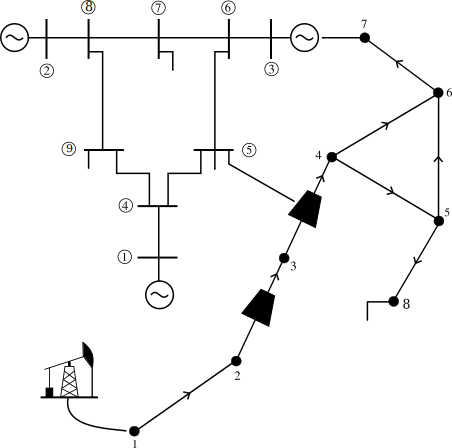
\includegraphics[scale=0.8]{Figures/Example1}
	\caption{Power and gas integrated network considered in Example 1.}
	\label{fig:example1}
\end{figure}


\begin{table}[!ht]
\centering
\begin{threeparttable}
\caption{Example 1 - Power System Summary}
\label{tab:ex1_power}
\footnotesize
\begin{tabular}{ll}
\toprule
\bf{topology}	& 9-bus network	 \\
\midrule
			& 3 gens at buses 1, 2, and 3\\
\bf{generators}	& 200 MW Max $P_{g}$ for all generators\\
			& all 3 have identical quadratic generation costs \tnote{*}\\
\midrule
\bf{load}		& 90 MW at bus 5, 100 MW at bus 7, 125 MW at bus 9 \\
			& curtailable at \$5000/MWh	\\
\midrule
\bf{branches}	& 250 MW limit for all lines	\\
\bottomrule
\end{tabular}
\begin{tablenotes}
 \scriptsize
 \item [*] {Linear costs of \$95/WMh are used for the example.}
\end{tablenotes}
\end{threeparttable}
\end{table}


\begin{table}[!ht]
%\renewcommand{\arraystretch}{1.2}
\centering
\begin{threeparttable}
\caption{Example 1 - Gas System Summary}
\label{tab:ex1_gas}
\footnotesize
\begin{tabular}{ll}
\toprule
\bf{topology}	& 8-node looped network	 \\
\midrule
			& 1 well at node 1\\
\bf{well}		& 80 MMSCF Max $g^{w}$ for well\\
			& linear cost extraction cost (\$5000 / MMSCFD )\\
\midrule
			& gas demands at nodes 7 and 8\\
\bf{load}		& 2 types of gas load 	\\
			& high cost of non-supplied demand\\
\midrule
\bf{pipelines}	& no active limits for all lines	\\
			& transport cost at (\$5 / MMSCFD) for all pipelines \\
\midrule
\bf{compressors}	& no active limits for all compressors	\\
			& transport cost at (\$5 / MMSCFD) for all compressors \\
\midrule
\bf{storage}	& no storage considered	\\			
\bottomrule
\end{tabular}
\begin{tablenotes}
 \scriptsize
 \item [] {}
\end{tablenotes}
\end{threeparttable}
\end{table}

Initially, for the sake of convenience and code portability, we define the column pointers (constants) for the power system\footnote{The default \matpower{} function \code{define\_constants} allows an straightforward indexing of all information via integer variables. See \cite{matpower_manual} for details.}. Similarly, we define column pointers to easily access the natural gas and interconnection cases, as follows:

\begin{Code}
>> define_constants        % power system constants
>> define_constants_gas    % natural gas system and connect struct constants
\end{Code}

We can load the \matpower{} options struct to chose the desired solver and some additional features. The current stable solver for \mpng{}  is `IPOPT'. Besides, based on the experience, we set the maximum number of iterations to 100000, as shown below:

\begin{Code}
>> mpopt = mpoption;                   % initialize option struct
>> mpopt.opf.ac.solver = `IPOPT';      % current stable solver
>> mpopt.ipopt.opts.max_iter = 1e5;    % max iterations
\end{Code}

Afterwards, we load the power and gas cases and the connection struct\footnote{All cases and connection struct are included in the folder \mpngcasepath{}. Since the data of the interconnection case mainly comprises additional information of the \matpower{}-case, we refer to the connect struct using a similar name as that used for the power system case.}. For the sake of simplicity, we name the power case as \code{mpc}, the natural gas case as \code{mgc},  and the connection struct as \code{connect}, as follows: 

\begin{Code}
>> mpc = loadcase(`case9_new');    % 9 bus power system
>> mgc = ng_case8;                 % 8 node natural gas system
>> connect = connect_pg_case9;     % interconnection case
\end{Code}

As the window of analysis consist in an entire day for the gas network, we just need to define the number of periods and their corresponding length for analyzing the power system. We consider four periods of time, each of them of the same length, that is:

\begin{Code}
>> connect.power.time = [6 6 6 6];   % four periods of time
\end{Code}

The connection struct also requires the active and reactive demands in all buses for each period. Then, we take the original system's demand to produce such a temporal behavior via a factor vector as follows:  

\begin{Code}
>> factors = [1 1.1 1.2 0.9];      % factors (external aid of MPNG)
>> connect.power.demands.pd = factors.*mpc.bus(:,PD);  % PD matrix
>> connect.power.demands.qd = factors.*mpc.bus(:,QD);  % QD matrix
\end{Code}

Moreover, we set the generator number two to have a maximum daily energy of 5000 MWh/d:

\begin{Code}
>> connect.power.energy = zeros(1,2);  % initialize (one gen with max energy)
>> connect.power.energy(1,GEN_ID) = 2;         % id for max energy in gen 2 
>> connect.power.energy(1,MAX_ENER) = 5000;    % max energy is 1000 MWh/d 
\end{Code}

For this particular example, we do not consider spinning reserve because of the small number of generators. As a consequence, the spinning reserve matrix is set to be an empty array:

\begin{Code}
>> connect.power.sr = [];                      % no spinning reserves
\end{Code}

As shown in Figure \ref{fig:example1}, both classes of compressors where included in this example. Their corresponding information, specified in the connection struct, must be consistent with the gas and power cases:

\begin{Code}
>> connect.interc.comp = zeros(1,2); % initialize (a power-driven compressor)
>> connect.interc.comp(1,COMP_ID) = 2;       % second compressor
>> connect.interc.comp(1,BUS_ID) = 5;        % connected to bus # 5
>> mgc.comp(2,TYPE_C) = COMP_P;              % concordance with gas case
\end{Code}

Additionally, a gas-fired power plant was considered, and its information must be included in the connection struct in a manner consistent with the gas and power cases:

\begin{Code}
>> connect.interc.term = zeros(1,3);       % initialize (one gas-fired plant)
>> connect.interc.term(1,GEN_ID)  = 3;     % third power plant
>> connect.interc.term(1,NODE_ID) = 7;     % connected to node # 7
>> connect.interc.term(1,EFF) = 10e-3;     % power plant eff. (MMSCFD/MWh)
\end{Code}

At this point, we have set all the inputs required to model the different aspects that we intended for the interconnected power and natural gas system. Now, we need to put all together in a single struct. We call this struct \code{mpgc}, which represents the combination between \code{mpc}, \code{mgc}, and \code{connect}, as shown below:

\begin{Code}
>> mpgc = mpc;                         % initialize MPNG case
>> mpgc.mgc = mgc;                     % adding gas case
>> mpgc.connect = connect;             % adding connection struct
\end{Code}

Finally, we can run the simulation by calling \mpng{} using the \code{mpgc} case and the \matpower{} options struct:
 
\begin{Code}
>> results = mpng(mpgc,mpopt);         % running simulation
\end{Code}

The optimal solution values are saved as the \code{results} struct.  See Section \ref{subsec:view_results} for more details about the simulation \code{results}. By default, the \code{results} are pretty-printed. The information related to the natural gas network after running the simulation looks like:\\

\vspace{-0.3cm}

%\begin{tiny}
%\begin{Code}
%		    >>  ================================================================================
%			|     Gas system summary                                                       |
%			================================================================================
%			
%			How many?                  How much?              
%			---------------------    -------------------------------- 
%			Nodes            8         Total Well Capacity    80.00 
%			Wells            1         On-line Capacity       80.00
%			Pipelines        6         Gas Production         45.83
%			Compressors      2         Total Demand           38.63
%			  Gas Comp.      1           Supplied Demand      38.63
%			  Power Comp.    1           Non-Supplied Demand  -0.00
%			Storage Units    1         Gas Stored             0.00
%			
%			Gas total extration cost =   229169.12
%			================================================================================
%			|     Nodes Data                                                               |
%			================================================================================
%			 Node   Pressure   Over      Under     Demand    Non-S       Gas        Nodal   
%			  #      (psi)    Pressure  Pressure  (MMSCFD)   Demand   Extraction    Lambda  
%			 ----   --------  --------  --------  --------  --------  -----------  ---------
%			   1     650.000     0.00      ---       ---       ---        45.83      5000.00 
%			   2     563.146     ---       ---       ---       ---         ---       5911.35 
%			   3     577.053     ---       ---       ---       ---         ---       5916.39 
%			   4     612.558     ---       ---       ---       ---         ---       6083.14 
%			   5     586.604     ---       ---       ---       ---         ---       6389.94 
%			   6     592.410     ---       ---       ---       ---         ---       6212.97 
%			   7     530.413     ---       ---      12.22     -0.00        ---       6217.97 
%			   8     464.000     ---       ---      26.41      0.00        ---       8019.82 
%			
%			================================================================================
%			|     Pipeline Data                                                            |
%			================================================================================
%			 Pipeline    From      To      Weymouth    Max Gas       Gas       Transport
%			    #        Node     Node     Constant     Flow         Flow       Cost    
%			 --------    -----    -----    --------    --------    --------    ---------
%			    1          1        2        0.141       80.00       45.83       229.17 
%			    2          4        5        0.121       40.00       21.42       107.09 
%			    3          4        6        0.157       40.00       24.42       122.08 
%			    4          5        6        0.060       40.00       -5.00        24.99 
%			    5          6        7        0.074       40.00       19.42        97.09 
%			    6          5        8        0.074       40.00       26.41       132.07 
%			
%			================================================================================
%			|     Compressor Data                                                          |
%			================================================================================
%			 Comp.   Comp.   From    To     Comp.      Power       Gas      Comp.    Comp.  
%			   #     Type    Node   Node    Flow      Consumed   Consumed   Ratio    Cost   
%			 -----   -----   ----   ----   --------   --------   --------   -----   --------
%			   1       G       2      3      45.834      1.29     0.0003    1.025   229.17
%			   2       P       3      4      45.834      3.17       ---     1.062   229.17
%			
%			================================================================================
%			|     Gas-fired Generators Data                                                |
%			================================================================================
%			 Unit.   Node   Plant       Daily      Gas                               
%			   #      #      Eff.       Energy    Consumed                           
%			 -----   ----  ---------   --------   --------                           
%			   3      7     1.00e-02     720.00      7.20
%			 -----   ----  ---------   --------   --------                           
%			                   Total     720.00      7.20   
%\end{Code}
%\end{tiny}


\begin{small}
\begin{Code}
    >>  ================================================================================
	|     Gas system summary                                                       |
	================================================================================
	
	How many?                  How much?              
	---------------------    -------------------------------- 
	Nodes            8         Total Well Capacity    80.00 
	Wells            1         On-line Capacity       80.00
	Pipelines        6         Gas Production         45.83
	Compressors      2         Total Demand           38.63
	Gas Comp.        1           Supplied Demand      38.63
	Power Comp.      1           Non-Supplied Demand  -0.00
	Storage Units    1         Gas Stored              0.00
	
	Gas total extraction cost =   229169.12
	================================================================================
	|     Nodes Data                                                               |
	================================================================================
	Node   Pressure     Over      Under    Demand     Non-S      Gas         Nodal   
	  #      (psi)    Pressure  Pressure  (MMSCFD)   Demand   Extraction    Lambda  
	----   --------  --------  --------  --------  --------  -----------  ---------
	  1     650.000     0.00      ---       ---       ---        45.83      5000.00 
	  2     563.146     ---       ---       ---       ---         ---       5911.35 
	  3     577.053     ---       ---       ---       ---         ---       5916.39 
	  4     612.558     ---       ---       ---       ---         ---       6083.14 
	  5     586.604     ---       ---       ---       ---         ---       6389.94 
	  6     592.410     ---       ---       ---       ---         ---       6212.97 
	  7     530.413     ---       ---      12.22     -0.00        ---       6217.97 
	  8     464.000     ---       ---      26.41      0.00        ---       8019.82
	================================================================================
	|     Pipeline Data                                                            |
	================================================================================
	Pipeline    From      To      Weymouth    Max Gas       Gas       Transport
	   #        Node     Node     Constant     Flow         Flow        Cost    
	--------    -----    -----    --------    --------    --------    ---------
	   1          1        2        0.141       80.00       45.83       229.17 
	   2          4        5        0.121       40.00       21.42       107.09 
	   3          4        6        0.157       40.00       24.42       122.08 
	   4          5        6        0.060       40.00       -5.00        24.99 
	   5          6        7        0.074       40.00       19.42        97.09 
	   6          5        8        0.074       40.00       26.41       132.07 	 
\end{Code}
\end{small}


\begin{small}
	\begin{Code}	
	================================================================================
	|     Compressor Data                                                          |
	================================================================================
	 Comp.   Comp.   From    To     Comp.      Power       Gas      Comp.    Comp.  
	   #     Type    Node   Node    Flow      Consumed   Consumed   Ratio    Cost   
	 -----   -----   ----   ----   --------   --------   --------   -----   --------
	   1       G       2      3      45.834      1.29     0.0003    1.025   229.17
	   2       P       3      4      45.834      3.17       ---     1.062   229.17
	
	================================================================================
	|     Gas-fired Generators Data                                                |
	================================================================================
	 Unit.   Node   Plant       Daily      Gas                               
	   #      #      Eff.       Energy    Consumed                           
	 -----   ----  ---------   --------   --------                           
	   3      7     1.00e-02     720.00      7.20
	 -----   ----  ---------   --------   --------                           
	                   Total     720.00      7.20   	
\end{Code}
\end{small}

\section{48-node Looped Natural Gas Network}
\label{sec:48_gas}

In this example, we show the capability of \mpng{} for solving looped natural gas systems. We highlight that \mpng{} is also a tool for analyzing independent natural gas networks. In particular, we can use a virtual two-bus power system as the power case just to allow \matpower{} to work properly. The information for the 48-node gas network considered in this example was provided by Cheng et al.~\cite{Chen2017}, whose topology is shown in Figure \ref{fig:ng48}.\\

\begin{figure}[H]
\centering
\includegraphics[scale=1.6]{Figures/NG48}
\caption{Natural gas network for Example 2. Source:~\cite{Chen2017}.}
\label{fig:ng48}
\end{figure}

In terms of computational and mathematical tractability, looped natural gas systems are the most complex to solve because they require nodal pressures that guarantee the gas flow in more than one pipeline~\cite{Woldeyohannes2011}. This states an interesting scenario to assess the performance of \mpng{}. In this example, we consider two case studies over the 48-node gas network: a \textit{base case} study, where elements interact properly in a normal operation with no perturbations; and a \textit{contingency case} study, where failures lead to complex decisions for the simulator.

Following Example \ref{sec:8-9_gas_power}, we start by defining all the power, gas, and connect constants. Then, we load the corresponding cases for this example: the gas case (\code{ng\_case48}), and the straightforward 2-bus power system (\code{case2}) that allows the virtual connection to the natural gas system (\code{connect\_pg\_case2}) with minimal implications in topological and computational terms. Lastly, we package the cases and the connect struct together and  run \mpng{}:

\begin{Code}
mpc = loadcase(`case2');        % 2 bus power system 
mgc = ng_case48;                % 48 node looped natural gas system
connect = connect_pg_case2;     % interconnection case

%% put cases together
mpgc = mpc;                     % initialize MPNG case
mpgc.mgc = mgc;                 % adding gas case
mpgc.connect = connect;         % adding connection struct

%% run mpng
res_base = mpng(mpgc,mpopt);         % running MPNG
\end{Code}

Now, we modify the base case to obtain the \textit{contingency case}. Specifically, we reduce the maximum injection capability of one of the wells located at the network center (node 20), forcing the system to extract natural gas from somewhere else to fulfill the gas demand. Moreover, we set pipeline number 38 (the one that connects nodes 43 and 44) to be out of service, eliminating one of the gas network loops located downstream. This contingency forces the system to supply the demands of nodes 30 to 33 through only two paths, which might cause over-pressures and pipeline congestion. 

To simulate these contingencies, we start again by loading the 48-node gas case. Then, we set the reduced maximum injection for well 9. For eliminating the mentioned pipeline, we remove its whole corresponding row in the field \code{mgc.pipe}. Once the contingencies are properly modeled, we put the entire system together and finally rerun the program:

\begin{Code}
%% changes due to contingencies
mgc_cont = mgc;
mgc_cont.well(9,GMAX) = 200;        % set max injection of well 9
cont_pipe = 39; 		    % id for out-of-service pipeline	 
mgc_cont.pipe(cont_pipe,:) = [];    % take pipeline out of service

%% putting all together
mpgc_cont = mpc;                    % initialize MPNG case
mpgc_cont.mgc = mgc_cont;           % adding gas case
mpgc_cont.connect = connect;	% adding connection struct

%% running program 
res_cont = mpng(mpgc_cont,mpopt);   % running MPNG
\end{Code}

Figures \ref{fig:ex2_pressure} to \ref{fig:ex2_inj} show the results comparison between the base case and the contingency case. We mainly analyze pressures, gas flows, and well injections, since they are the most representative variables in the gas network. As seen, reducing the injection capacity in node 22 leads not only to the maximum injection in node one but also to the activation of the wells located at nodes 2 and 6 to balance the global production. As a consequence, new gas flows appear through pipelines 4-7 and 6-7 as a result of higher pressures in nodes 2 to 7; moreover, the gas flow through pipe 1-8 increases at the expense of lower pressure of node 8. Besides, compressors 1, 2, and 3 are forced to transport larger flows by increasing the difference between suction and discharge pressures, that is, their compressor ratios. On the other hand, the outage of pipeline 43-44 leads to higher pressures in the surrounding nodes because of the new radial connections of some pipes. Notice how pipelines 36-43 and 43-42 end up with gas flows in the opposite direction in the contingency case.

\begin{figure}[H]
\centering	
\includegraphics[scale=0.8]{Figures/ex2_pressure}
\caption{Results Example 2 - Nodal Pressure.}
\label{fig:ex2_pressure}
\end{figure}

\begin{figure}[H]
\includegraphics[scale=0.75]{Figures/ex2_fgo}
\caption{Results Example 2 - Gas Flow Through Pipelines.}
\label{fig:ex2_fgo}
\end{figure}

\begin{figure}[H]
\centering
\includegraphics[scale=0.8]{Figures/ex2_fgc}
\caption{Results Example 2 - Gas Flow Through Compressors.}
\label{fig:ex2_fgc}
\end{figure}

\begin{figure}[H]
\centering
\includegraphics[scale=0.8]{Figures/ex2_inj}
\caption{Results Example 2 - Gas Injection in Wells.}
\label{fig:ex2_inj}
\end{figure}


	
\end{document}